\documentclass[a4paper, 12pt]{article}
\usepackage[utf8]{inputenc}
\usepackage[T1]{fontenc}
\usepackage[french]{babel}
\usepackage{lmodern}
\usepackage{graphicx, float, svg} 
\usepackage{amsmath, amssymb, amsthm}
\usepackage{listings}
\usepackage[listings,skins]{tcolorbox}
\usepackage{xcolor}

\usepackage[hyphens]{url}
\usepackage[pdfauthor = {{Prénom Nom}}, pdftitle = {{Titredocument}},pdfstartview = Fit, pdfpagelayout =
SinglePage, pdfnewwindow = true, bookmarksnumbered =
true, breaklinks, colorlinks, linkcolor = red, urlcolor =
black, citecolor = cyan, linktoc = all]{hyperref}

\usepackage[a4paper,margin=2.5cm]{geometry}

% \renewcommand{\familydefault}{\sfdefault}
\definecolor{codegreen}{rgb}{0,0.6,0}
\definecolor{codegray}{rgb}{0.5,0.5,0.5}
\definecolor{codepurple}{rgb}{0.58,0,0.82}
\definecolor{codeblue}{rgb}{0.0, 0.4, 0.8}
\definecolor{darkWhite}{rgb}{0.90,0.90,0.90}

\lstdefinestyle{bigCode}{
    backgroundcolor=\color{darkWhite},   
    commentstyle=\color{codegreen},
    keywordstyle=\color{codeblue},
    numberstyle=\tiny\color{codegray},
    stringstyle=\color{codepurple},
    basicstyle=\ttfamily\footnotesize,
    breakatwhitespace=false,         
    breaklines=true,                 
    captionpos=b,                    
    keepspaces=true,                 
    showspaces=false,                
    showstringspaces=false,
    showtabs=false,                  
    tabsize=2,
    language=c,
    morekeywords={free,malloc,nullptr,calloc,memcpy,realloc,bool,size_t,true,false}
}

\lstset{style=bigCode}

\NewTotalTCBox{\commandbox}{ s v }
{verbatim,colupper=black,colback=darkWhite!75!white,colframe=white,left=0pt,boxsep=0px,right=0pt,top=2px,bottom=2px}
{\IfBooleanT{#1}{\textcolor{red}{\ttfamily\bfseries > }}%
\lstinline[language=c,morekeywords={free,malloc,nullptr,calloc,memcpy,realloc,bool,size_t,true,false},keywordstyle=\color{codeblue}\bfseries]^#2^}

\newcommand{\code}{\commandbox}

\title{Distance de Jaccard}
\author{Maysaloon BILAL \& Tristan GROULT}
\date{\today}

\begin{document}

\begin{figure}[t]
    \centering
    \begin{minipage}{0.3\textwidth}
        \centering
        
\includegraphics[width=1\textwidth]{logo_univ.png}
    \end{minipage}
    \hfill
    \begin{minipage}{0.3\textwidth}
        \centering
        
\includegraphics[width=1\textwidth]{ufr_logo.png}
    \end{minipage}
\end{figure}

\maketitle

\clearpage\setcounter{page}{2}

{
\hypersetup{hidelinks} % Sommaire en "noir"
\renewcommand{\contentsname}{Sommaire}
\tableofcontents % Affichage du sommaire
}

\clearpage

\section{Introduction}


Ce projet consiste à développer un programme en langage C permettant de calculer la distance de Jaccard entre plusieurs fichiers texte, afin d’analyser leur similarité lexicale. La distance de Jaccard est une valeur comprise entre 0 et 1 : plus elle est proche de 0, plus les fichiers sont différents, et plus elle est proche de 1, plus ils sont similaires.

La distance de Jaccard entre deux ensembles $A$ et $B$ est définie par la formule :
$$
\text{Distance de Jaccard}(A, B) = 1 - \frac{|A \cap B|}{|A \cup B|}
$$

Le programme permet plusieurs personnalisations. Il est possible d’afficher un graphe indiquant à quels fichiers chaque mot appartient, ou d’activer un mode détaillé qui précise pour chaque mot les fichiers dans lesquels il apparaît. Une autre option permet également de définir une longueur maximale pour les mots analysés.

Pour gérer efficacement les mots extraits des fichiers, nous avons utilisé une table de hachage. Sa gestion — ajout, suppression, affichage du graphe, etc. — est implémentée dans le module \code{jaccard}. Ce projet s’appuie également sur deux autres modules : le module \code{word}, dédié à la création et la manipulation des mots, et le module \code{opt}, responsable du traitement des options en ligne de commande.

L’ensemble de ces composants est intégré et testé dans le fichier principal \code{main.c}, qui constitue le point d’entrée du programme.


\section{Méthodologie}

Dans cette section, nous expliquons les différentes étapes et approches utilisées pour implémenter le programme. Nous détaillerons la conception des modules, la gestion des fichiers et l’utilisation de la table de hachage.

\subsection{Module word}

Le module \code{word.c} sert à construire dynamiquement un mot caractère par caractère. Il est composé de 3 champs : 
\begin{itemize}
  \item Un champ \code{s} de type \code{char *} qui pointe vers un tableau de caractères qui stocke le mot lui-même.
  \item Un champ \code{length} de type \code{size_t } qui représente la longueur du mot.
  \item Un champ \code{capacity} de type \code{size_t} qui représente la capacité du tableau pointé par \code{s}
\end{itemize}



\begin{figure}[h]
\centering
\begin{tcolorbox}[center upper,
    enhanced,
    colback=darkWhite,
    boxrule=0pt,
    frame hidden,
    width=0.4\textwidth]
\begin{lstlisting}[style=bigCode]
struct word {
    char *s;
    size_t length;
    size_t capacity;
}; 
\end{lstlisting}
\end{tcolorbox}
    \caption{Structure word}
    \label{fig:structure_word} 
\end{figure}



\begin{itemize}
    \item \textbf{Initialisation d’un mot} : La fonction \code{word_init()} permet de créer un nouveau mot avec une capacité initiale minimale définie par la constante \code{CAPACITY_MIN}. Elle alloue dynamiquement de la mémoire pour la chaîne de caractères et initialise sa longueur à zéro.
    
    \item \textbf{Ajout d’un caractère au mot} : La fonction \code{word_add()} ajoute un caractère à un mot. Si le mot atteint sa capacité maximale, la fonction double l'espace mémoire disponible avec \code{realloc()}, pour permettre l'ajout de nouveaux caractères. Cela permet au programme de gérer des mots de tailles variables sans perdre de données.
    
    \item \textbf{Réinitialisation du mot} : La fonction \code{word_reinit()} permet de réinitialiser un mot, c'est-à-dire de remettre sa longueur à zéro et de vider la chaîne. Cela est utile lorsqu'un mot doit être réutilisé sans allouer de mémoire supplémentaire.
    
    \item \textbf{Accès à la chaîne de caractères} : La fonction \code{word_get()} renvoie un pointeur vers la chaîne, tandis que \code{word_get_clean()} copie le mot dans dest, permettant ainsi de ne récupérer que le mot réel, sans les parties inutilisées de la mémoire allouée. Cela garantit que le mot est prêt à être utilisé sans risque de contenir des espaces "vides" dans la mémoire.
\end{itemize}



\begin{figure}[H]
    \centering
    \begin{tcolorbox}[enhanced,
        colback=white,
        colframe=codeblue,
        fonttitle=\bfseries,
        title=Schéma,
        boxrule=2pt,
        width=0.8\textwidth]
        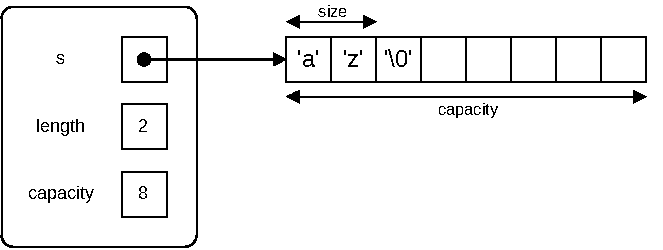
\includegraphics[width=\textwidth]{word_schema.pdf}
    \end{tcolorbox}
    \caption{Schéma de la structure word}
    \label{fig:word_schema}
\end{figure}



\subsection{Module opt}

Le module \code{opt} a pour objectif de gérer facilement les options lue sur la ligne de commande afin de les annlyser et de le retranscrire dans une forme utilisable. Pour ce projet, nous avons beson des options suivante :

\begin{itemize}
    \item Une option permettant la demande d'affichage du graphe de Jaccard.
    \item Une option permettant d'ignoré les caractères de ponctuations.
    \item Une option permettant de majoré la longueur des mots.
    \item Une option permettant d'utiliser l'entré standard comme source.
    \item Une option permettant de définir le prochain élément comme le nom d'un fichier.
    \item Une option permettant d'afficher comment utiliser l'exécutable.
    \item Une option permettant d'afficher la version de l'exécutable.
    \item Une option permettant d'afficher l'aide de l'exécutable.
\end{itemize}

\subsubsection{Spécification}

Pour cella, nous utilisont une structure de donné définie par le shéma de la \autoref{fig:opt_schema}. Nous avons choisit de limiter le nombre de fichier à une constantante nomé ici \texttt{max files} afin de bénéficiait d'un temps et espace constant. Cepandant, ce choix est aussi utile pour les choix d'implémentations que nous nous sommes fixé pour le module \code{jaccard}.

\begin{figure}[H]
    \centering
    \begin{tcolorbox}[enhanced,
        colback=white,
        colframe=codeblue,
        fonttitle=\bfseries,
        title=Schéma,
        boxrule=2pt,
        width=0.8\textwidth]
        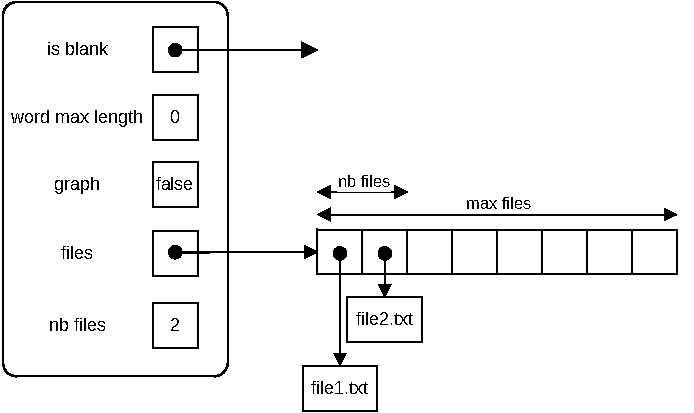
\includegraphics[width=\textwidth]{opt_schema.pdf}
    \end{tcolorbox}
    \caption{Schéma de la structure word}
    \label{fig:opt_schema}
\end{figure}

\subsubsection{Implantation}

Lors de l'implémantation, nous avons choisit d'utiliser un \code{struct} (\autoref{fig:structure_opt}) pour représenter notre structure de donnés.
Nous avons aussi choisi de sauvgarder l'utilisation de l'entré standard de la même manière que pour les fichiers en définisant grâce à une macro constante nomé \code{STDIN} la valeur spécifique \code{""} qui est la chaine vide car aucun systheme majeure authorsise cette valeur comme nom de fichier. Cette structure est composé de 5 champs:

\begin{itemize}
    \item Un champ \code{isBlank} de type \code{int (*)(int)} qui définie la fonction déterminant les caractère séparant les mots.
    \item Un champ \code{word_max_length} de type \code{int} qui définie le nombre de caratères maximum composant un mot. Si cette valeur vaut 0, alors aucune limitations sur la taille du mot n'est appliqué, ça valeur par défaut est 0.
    \item Un champ \code{graph} de type \code{bool} qui définie si l'utilisateur demande l'affichage du graph de Jaccard ou non.
    \item Un champ \code{files} de type \code{const char **} qui définie les nom des fichiers à traiter.
    \item Un champ \code{nb_files} de type \code{int} qui définie le nombre de fichiers spécifiait.
\end{itemize}

\begin{figure}[h]
\centering
\begin{tcolorbox}[center upper,
    enhanced,
    colback=darkWhite,
    boxrule=0pt,
    frame hidden,
    width=0.5\textwidth]
\begin{lstlisting}[style=bigCode]
struct opt {
    int (*isBlank)(int);
    int word_max_lenght;
    bool graph;
    char const **files;
    int nb_files;
}; 
\end{lstlisting}
\end{tcolorbox}
    \caption{Structure opt}
    \label{fig:structure_opt} 
\end{figure}

Nous avons fait le choix de dévelopé uniqument les options courtes pour les options sont énéoncé si dessous. Les options sont noté respectivement :

\begin{itemize}
    \item L'option est noté \code{-g}.
    \item L'option est noté \code{-p}.
    \item L'option est noté \code{-iVALUE}.
    \item L'option est noté \code{-}.
    \item L'option est noté \code{--}.
    \item L'option est noté \code{-u}.
    \item L'option est noté \code{-v}.
    \item L'option est noté \code{-?}
\end{itemize}

Nous pouvons remarquer que pour l'option \code{-iVALUE}, \code{VALUE} est collé au \code{-i}. Celle signifie que cette options fonctionne uniquement dans ce cas. Par exemple \code{-i3} est correct à l'inverse de \code{-i 3}.

Finalement, nous avons aussi fait le choix de rendre le codage de nos options facilemnt adaptatif en définisant toutes nos options grâce à des macro constante mais aussi en définisant séparément le préfix signifiant une option courte pour que n'importe qu'elle valeurs puisse être utilisé dans nos macros.





\end{document}